%!TEX root = ../template.tex
%%%%%%%%%%%%%%%%%%%%%%%%%%%%%%%%%%%%%%%%%%%%%%%%%%%%%%%%%%%%%%%%%%%%
%% chapter4.tex
%% NOVA thesis document file
%%
%% Chapter with lots of dummy text
%%%%%%%%%%%%%%%%%%%%%%%%%%%%%%%%%%%%%%%%%%%%%%%%%%%%%%%%%%%%%%%%%%%%
\chapter{Background}
\label{cha:background}
After the presentation of the problem and the motivations behind it, in this chapter will be introduced key concepts of Human-Computer Interaction, as well as, a briefly contextualization of the OutSystems Platform Background that are indispensable for the comprehension and progression of this study.

\section{Human-Computer Interaction}
\label{sec:human_computer_interaction}
Since the goal of this project is to improve and extend the visual language that gives to the user the possibility to construct queries through manipulation of visual components of graphical user interface. Human-computer interaction concepts, rules and techniques are fundamental to design and evaluate any possible solution to this problem. Thus, following, will be presented a summary of human-computer interaction topics taken into account throughout the design and development of this project.

Although computer systems have been designed by humans, these two parts of human-computer interaction do not communicate through the same language. Nonetheless, these type of systems were created to support, in a transparent way, human’s tasks and requirements, forgiving careless mistakes. \cite{humanComputerInteraction} Thus, human-computer interaction fields aim to study the relationship of users and computer systems, in the context of the users’ desired tasks, in order to “unfold and reveal challenges and insights, and to instrument appropriate solutions for alleviating the current obstacles to the access and use of advanced information technologies” \cite{userInterfacesForAll_newPerspectivesIntoHumanComputerInteraction}. 

%\textit{Dix et al.} \cite{humanComputerInteraction} reinforce this too, saying that “HCI involves the design, implementation and evaluation of interactive systems in the context of the user’s task and work”.

\subsection{Interaction Models}
\label{subsec:interaction_models}

Therefore, have been proposed interaction models to represent the intention of a user to perform a certain task on a system. One of the most influential is Norman’s model, that characterize the interaction of a user with a system beyond execution-evaluation cycles. \cite{humanComputerInteraction} Thereby, the execution is a flow when the user interacts with the system, and the evaluation phase comprise the presentation and the interpretation of the system output. However, this model only represents the interaction from the users’ point of view. Thereupon, Abowd and Beale \cite{userSystemsAndInterfaces_aUnifyingFrameworkForInteraction} proposed an extension of this model where it is possible to view how the system communicates through the interface.

In this approach, represented in Figure \ref{fig:abowdAndBealeModel}, after the user has defined his goal and respective tasks to achieve it, he transmits his intention (articulation) through input language, and after this, that information is translated to system language (performance), ending the execution phase. Secondly, the result of the action executed by the system is presented (presentation) and the user observes it (observation), ending the evaluation phase.

\begin{figure}[htbp]
	\centering
	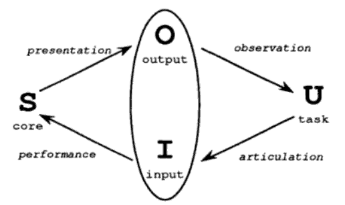
\includegraphics[height=1.75in]{abowdAndBealeModel}
	\caption{Interaction Model proposed by Abowd and Beale \cite{userInterfacesForAll_newPerspectivesIntoHumanComputerInteraction} (Based on Norman’s Model)}
	\label{fig:abowdAndBealeModel}
\end{figure}

These models are useful to understand two concepts that cannot be forgotten when a system is being designed, since these are two effects that designers want to reduce as much as possible, in order to optimize the effectiveness of the human-computer dialogue. Following, these concepts will be described respecting \textit{Dix et al.} \cite{humanComputerInteraction} definition:

\begin{itemize}
    \item \textbf{Gulf of execution}: “Difference between the user’s formulation of the actions to reach the goal and the actions allowed by the system. If the actions allowed by the system correspond to those intended by the user, the interaction will be effective.”
    \item \textbf{Gulfs of evaluation}: “Distance between the physical representation of the system state and the expectation of the user. If the user can readily evaluate the presentation in terms of his goal, the gulf of evaluation is small.”
\end{itemize}

\subsection{Main Concepts}
\label{subsec:main_concepts}
The \textbf{Usability} of a system is one of the most important concepts in human-computer interaction, that can not be forgotten on the design process, since its attributes must be taken into account performing also a guidance function through all this process. This concept was standardized in ISO-9241 \cite{iso9241-11_2018} as “extent to which a system, product or service can be used by specified users to achieve specified goals with effectiveness, efficiency and satisfaction in a specified context of use”.

However, usability is not a single-dimensional property, being always associated with its attributes, that characterize the user accessibility when is using the system into five different points, such as referred by Nielsen \cite{usabilityEngineering}:

\begin{itemize}
	\item \textbf{Learnability}: How easy is the learning process until a novice user (has not used the system before) has some high-level of proficiency using the system \cite{measuringLearnabilityInHumanComputerInteraction}. The learnability is higher as the learning process is faster, and the user has to spend less effort to reach his goal. Also, it depends on tutorials and training provided to users. A system that requires less training has a higher learnability than a system that requires more training. The time that a novice user requires to perform some specific tasks can be used to measure learnability. Learnability can be improved using tips while a novice user explores the system doing his first tasks.
	\item \textbf{Efficiency}: Refers to the productivity level of a user which have already learnt how to use the system. Efficiency can be measured analysing the time that expert users spent to do specific tasks on the system. This attribute can be improved, for example, adding shortcuts to accelerate the interaction process.
	\item \textbf{Memorability}: Defines how easy is for a user, that was using a system before but did not use it for a time period, to do his desired tasks on the system. So it’s related to how many time the user has not used the system and the time that the user needs to remember how the system works. Therefore, if a system has a good memorability the user does not need many time to remember it, even if it has stopped use it for a long period of time. Memorability can be measured, for example, analysing the interaction process of a user who has been away from the system, while he uses the system again. The use of visual components and metaphors with real-life objects helps, sometimes, the users in this process.
	\item \textbf{Errors}: A system not only must have a low error-rate but only if an error occurs, the user should be able to recover from that. Since there are multiple types of error with different severity levels, it is important that catastrophic errors must not occur. This attribute can be measured evaluating the error-rate, taking into account the severity levels of the errors. Furthermore, if a system has errors, that can be reverted and do not have a negative impact on the final result, cannot be forgotten that these errors also harm the efficiency of the system.
	\item \textbf{Satisfaction}: The most subjective attribute of the usability that is related to the overall satisfaction of the user when uses the system. Could be measured by asking the users about the experience while they are using the system, always searching for subjective answers.
\end{itemize}

Nonetheless, as mentioned by Nielsen \cite{usabilityEngineering}: 

\begin{center}
	\textbf{“it is not always possible to achieve optimal scores for all usability attributes simultaneously”}.
\end{center} 

Thus, when a system is designed it is necessary to prioritize what are the most important attributes for the users and the domain where the system will be used and applied. These trade-offs are one of the most challenging tasks of the design processes because it depends on user expectations and their backgrounds, as well as, the problem domain and what are the main focus of the system use.

Accordingly, it is fundamental that the design process can focus on target users of the systems. Therefore, following will be described some main concepts, processes and techniques for a design process centered on the users.

\subsection{User-centered Design}
\label{subsec:user_centered_design}
Before user-centered design principles and methodologies were adopted, the Waterfall model was commonly adopted as a software development process. This model comprises five sequential phases, from the requirements specification phase to the operation and maintenance phase, and has a good quality control since documentation and planning are a major concern of this methodology.\cite{aComparisonBetweenThreeSDLCModelsWatterfallSpiralIncrementalIterative} However, the stages of this model are not overlapping stages, so other development methodologies and philosophies arose to mitigate this problem and include the user on the design process, due to their impact on the usability of the system.

Consequently, it was necessary a new model that has the users included on the development process to verify, along the development, if the approaches adopted are positive and what is the users' acceptability. Nielsen \cite{iterativeUserInterfaceDesign} reinforces this saying that “user interfaces should be designed iteratively in almost all cases because it is virtually impossible to design a user interface that has no usability problems from the start. Even the best usability experts cannot design perfect user interfaces in a single attempt, so a usability engineering lifecycle should be built around the concept of iteration”.

The Spiral model of iterative design arose as an iteration through design, implementation and evaluation phases where the cost and accuracy increase on each iteration, since first iterations should use low-cost resources, like paper prototypes, and when the results are positive the accuracy is incremented, changing to computer prototypes, for example. \cite{interactionDesign_beyondHumanComputerInteraction} An overview of this model is represented in  Figure \ref{fig:spiralModel}.

\begin{figure}[htbp]
	\centering
	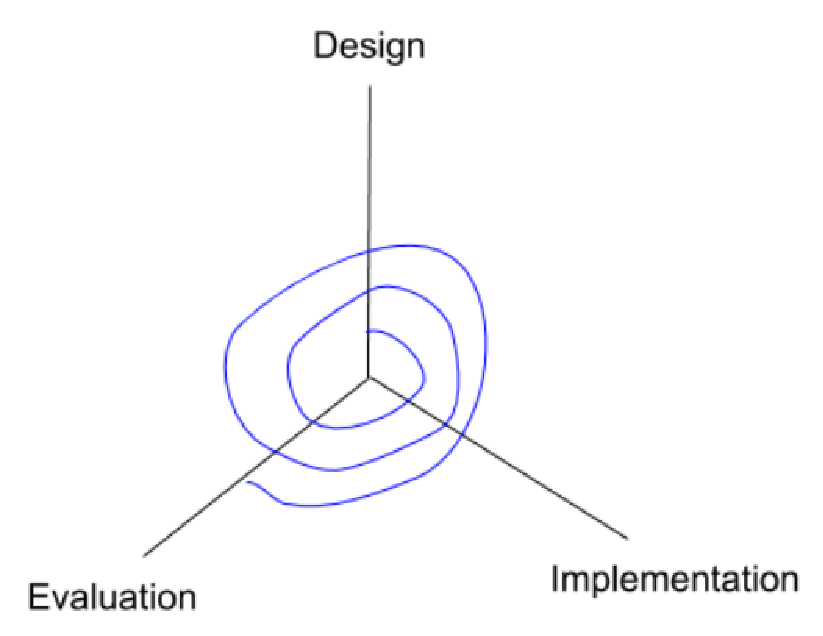
\includegraphics[height=1.75in]{spiralModel}
	\caption{Sprial model of Iterative Design (adapted from \cite{interactionDesign_beyondHumanComputerInteraction})}
	\label{fig:spiralModel}
\end{figure}

\subsubsection{User and Task Analysis}
\label{subsubsec:user_and_task_analysis}
Regarding the concept of usability presented above and the importance of the users on the design process, it is important to define the users and their desired tasks of the system in order to find the best solution as possible to the usability attributes trade-offs. Just a good description of the users and the tasks of the system leads the designers to the best choice of what are the usability attributes most important for the system.

Accordingly, it is important to make a \textbf{User Analysis} to understand all users’ characteristics that could have an impact on the acceptability of the system. The expected result of this analysis should be a set of structured information that characterize the users of the system in terms of technological expertise, knowledge of business domain, application experience, educational background, gender and age, as other aspects that might be useful to comprehend, depending on the system’s users and domain. \cite{userAnalysisInHCI_theHistoricalLessonFromIndividualDifferencesResearch} The more traditional process to gather this information is through questionnaires or interviews, but that can be obtained also beyond market analyses or observational studies. \cite{usabilityEngineering}

Furthermore, it is essential to enumerate and analyse the tasks the users should perform using the system. The \textbf{Task Analysis} process aims to aggregate information about the tasks that the system should perform, starting from the system overall goals and break down these to obtain individual tasks. \cite{usabilityEngineering} Moreover, the goal of this analysing process is to obtain more structured information about: how the tasks are performed using the existing systems, what are the pre-conditions and the requirements of each task, why the users need to perform this tasks, and others that might be useful to characterize the tasks of the system. 

The techniques used, to extract information to this analysis, tries that users specify how the tasks should be done instead of how they are done, resorting on examples as well as possible, in order to understand what type of strategies are used, what type of exceptions from their normal workflow are occurring, and other aspects that can be observed where the communication with users is on a concrete level, presenting also practical examples. \cite{usabilityEngineering} In addition, Nielsen \cite{usabilityEngineering} points out that  “The users' model of the task should also be identified, since it can be used as a source for metaphors for the user interface”, which reinforces that these dialogues with users to obtain analysis content, can be useful also to find relevant solutions to latter design process phases.

Therefore, the outcome of this analysis should contain a list of the entire tasks that users what to perform in the system, the information that is required to complete them, the steps and the dependencies between tasks, all the outputs that must be generated, and how is the communication process between the users associated with the system’s tasks. \cite{usabilityEngineering}


\subsubsection{Sketching and Prototyping}
\label{subsubsec:sketching_and_prototyping}
After the user and task analysis process, the designers must be able to start sketching and prototyping ideas and approaches in order to think about how can they solve the problems. Nevertheless, this phase of the design process should start with sketching techniques, as these are not only a good and inexpensive starting point to communicate ideas, but also help to develop structure and enrich the reasoning, leading to the perception of other details as well as of other approaches to solve the related problems.

While sketching techniques are more plentiful, and have a low detail level, suggesting and exploring rather than retrieving results, the prototyping phases, have more refinement approaches and are used to test the design choices made.

However, there are prototypes with different thoroughness degrees, presenting different advantages and disadvantages. Thus, it is important to start the prototyping process with low fidelity prototypes, as paper prototypes, since the objective of these is to evaluate the conceptual model (if the users understand the system), the functionalities presented, the navigation, the screen components distribution, and the terminology used. After the evaluation of these prototypes presents good results, high fidelity prototypes should be used, like computer prototypes. There are a set of available tools to assist in the building process of these prototypes, such as Balsamiq \cite{balsamiq} and Mockingbird \cite{mockingbird}. These different prototype types can detect different issues when tested with users, so it is very important to test prototypes with different granularity levels.

Furthermore, there is another relevant aspect of the prototype designing, that is the scope definition of the prototype. It is important to define what features the prototype undertakes and what is the inherent detail level. Nielsen \cite{usabilityEngineering} describe this as two dimensions of prototyping: horizontal prototyping and vertical prototyping, as demonstrated in Figure \ref{fig:prototypeDimensions}. A vertical prototype is characterized as a prototype to test a restricted part of the system but with real users and circumstances. A horizontal prototype is presented as suitable for test the entire system but in a less realistic approach.

\begin{figure}[htbp]
	\centering
	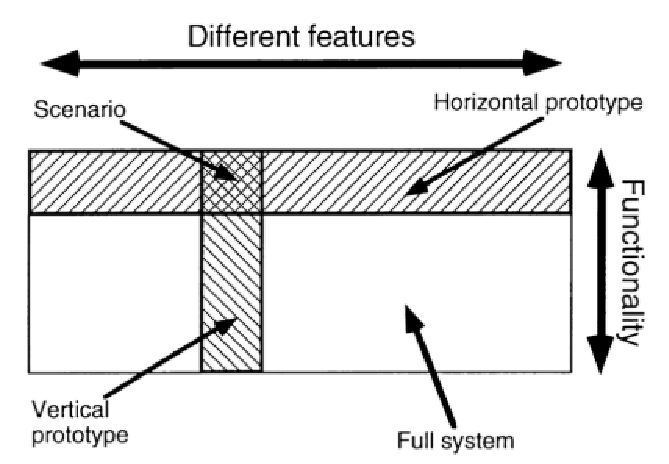
\includegraphics[height=2.5in]{prototypeDimensions}
	\caption{The two dimensions of prototyping: Horizontal prototyping keeps the features but eliminates depth of functionality, and vertical prototyping gives full functionality for a few features (extracted from \cite{usabilityEngineering})}
	\label{fig:prototypeDimensions}
\end{figure}

Finally, regarding the methodology about how to use the prototypes built, Dix et al. \cite{humanComputerInteraction} refer that are three main approaches:

\begin{itemize}
	\item \textbf{Throw-away}: After the prototype is built and tested, this is used on the final system development, but after this, the prototype built is discarded and the rest of the design process continues;
	\item \textbf{Incremental}: First, the system is separated into different parts, and each part is built, one at a time. So the prototypes are developed separately, regarding its correspondent part, and finally are combined together to build the final system;
	\item \textbf{Evolutionary}: Contrary as throw-away approach, the prototypes developed are used as the basis for the next iteration of design.
\end{itemize}





\subsubsection{Evaluation Techniques}
\label{subsubsec:user_and_task_analysis}

\subsubsection{Errors Classification}
\label{subsubsec:errors_classification}
The errors occurred when a users interacts with a system are an excellent indicator to designers. Thus, what reason led the user to reach the error, is a good strategy to understand and classify them. Therefore, errors can be classified as slips and mistakes, as will be presented below according to Dix \textit{et al.} \cite{humanComputerInteraction}:

\begin{itemize}
	\item \textbf{Slips}: in these type of errors, the user knows how to do the pretended task on the system, however, he presses a wrong button or closes one window accidentally. So, he understands the action, but a misaction does not permit that he reaches his goal;
	\item \textbf{Mistakes}: these errors occur when the user does not understand the system, formulating a wrong goal. An example of an Mistake is when the user does not understand the action associated with an icon, performing a not pretended action.
\end{itemize}

Therefore, the strategy to mitigate the problems associated with these two types of errors could be different, as mentioned by Dix \textit{et. al.} \cite{humanComputerInteraction}: “Slips may be corrected by, for instance, better screen design, perhaps putting more space between buttons. However, mistakes need users to have a better understanding of the systems, so will require far more radical redesign or improved training, perhaps a totally different metaphor for use.”


\section{OutSystems Background}
\label{sec:outsystems_background}

\subsection{Platform Overview}
\label{subsec:platform_overview}

\begin{figure}[htbp]
	\centering
	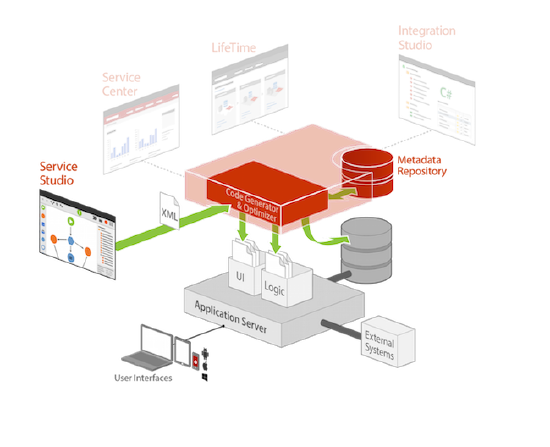
\includegraphics[height=3.75in]{outsystemsArchitecture}
	\caption{OutSystems Platform Overview \cite{outsystemsToolsAndComponents}}
	\label{fig:outsystemsArchitecture}
\end{figure}

\subsection{Previous Work}
\label{subsec:previous_work}
